

\documentclass[xcolor=dvipsnames]{beamer}

\usetheme[left]{Goettingen}

\newcommand{\denselist}{\itemsep 0pt\partopsep 0pt}
\usepackage{tipa}
\usepackage[square,sort,comma,numbers]{natbib}
\usepackage{graphicx}
\graphicspath{{images/}}
\usepackage[font={scriptsize,it}]{caption}

\newcommand{\g}{\,\vert\,}

\newcommand{\ent}{\textrm{H}}
\newcommand{\likelihood}{\ell}
\newcommand{\mn}{\textrm{MN}}
\newcommand{\mult}{\textrm{Multinomial}}
\newcommand{\dir}{\textrm{Dir}}
\newcommand{\poiss}{\textrm{Poisson}}
\newcommand{\vocab}{{\cal V}}
\newcommand{\E}{\textrm{E}}
\newcommand{\data}{{\cal D}}
\newcommand{\p}{p}
\newcommand{\q}{q}
\newcommand{\dhat}{d}
\newcommand{\dataset}{{\cal D}}
\newcommand{\fracpartial}[2]{\frac{\partial #1}{\partial  #2}}
\newcommand{\w}{\textbf{w}}
\newcommand{\z}{\textbf{z}}
\newcommand{\Th}{{\textrm{th}}}
\newcommand{\diag}{\textrm{diag}}
\newcommand{\one}{\textbf{1}}
\newcommand{\onet}{\textbf{1}^{\textrm{T}}}
\newcommand{\kl}{\textrm{D}}

\newcommand{\mysec}[1]{Section~\ref{sec:#1}} 
\newcommand{\myapp}[1]{Appendix~\ref{app:#1}} 
\newcommand{\myeq}[1]{Eq.~(\ref{eq:#1})}
\newcommand{\myeqp}[1]{Eq.~\ref{eq:#1}}

\newcommand{\textsum}[3]{\textstyle\sum_{#2=1}^{#3} #1_{#2} \displaystyle}
\newcommand{\textsumsuper}[3]{\textstyle\sum_{#2=1}^{#3} #1^{#2} \displaystyle}
\newcommand{\basictextsum}[3]{\textstyle\sum_{#2=1}^{#3}#1\displaystyle}

\newcommand{\source}[1]{\caption*{Source: {#1}} }

\title{Generating Natural Questions About an Image}

% A subtitle is optional and this may be deleted
\subtitle{\cite{mostafazadeh-EtAl:2016:P16-1}}

\author{Ryan Callihan \& Sarah Taylor}
% - Give the names in the same order as the appear in the paper.
% - Use the \inst{?} command only if the authors have different
%   affiliation.

\institute[Universit{\"a}t T{\"u}bingen] % (optional, but mostly needed)
{
	%
	Seminar f{\"u}r Sprachwissenschaft\\
	Universit{\"a}t T{\"u}bingen
}
% - Use the \inst command only if there are several affiliations.
% - Keep it simple, no one is interested in your street address.

\date{Janurary 12, 2018}
% - Either use conference name or its abbreviation.
% - Not really informative to the audience, more for people (including
%   yourself) who are reading the slides online

\subject{Question Generation | Winter 17/18}
% This is only inserted into the PDF information catalog. Can be left
% out. 

% If you have a file called "university-logo-filename.xxx", where xxx
% is a graphic format that can be processed by latex or pdflatex,
% resp., then you can add a logo as follows:



% Delete this, if you do not want the table of contents to pop up at
% the beginning of each subsection:

% Let's get started
\beamertemplatenavigationsymbolsempty 

\setbeamercolor{structure}{fg=black}



\makeatletter
\setbeamertemplate{sidebar canvas \beamer@sidebarside}[vertical shading][top=red!190, bottom=BrickRed!190]
\makeatother

\addtobeamertemplate{navigation symbols}{}{%
	\usebeamerfont{footline}%
	\usebeamercolor[fg]{footline}%
	\hspace{1em}%
	\insertframenumber/\inserttotalframenumber
}


\makeatletter

\begin{document}
	
	\begin{frame}
		\titlepage
	\end{frame}
	
	\begin{frame}{Outline}
		\tableofcontents
	\end{frame}
	
	%TODO Introduction - separate into groups and call and response - BOTH
	\section{Generating Questions from Pictures}
	
		\begin{frame}
			\frametitle{Getting Started}
			Make groups!
		\end{frame}
	
		\begin{frame}
			\frametitle{Challenge One - Setup}
			Please go to: and enter in the code:
		\end{frame}
		
		%ritual | Is this a religious ceremony?---That looks very interesting, don't you think?---What are they all gathered for?---What are these people gathered for?---Is this a satanic ritual?	| A group of people are gathered outside a statue outside---A stone temple statue with a fire burning at it's base, people are standing on the stairs beneath it---People standing in front of a bonfire on an alter---People surround a large fire---A religious ceromony of some sort is being celebrated with a bonfire in front of a large statue.
		
		\begin{frame}
			\frametitle{Challenge One}
			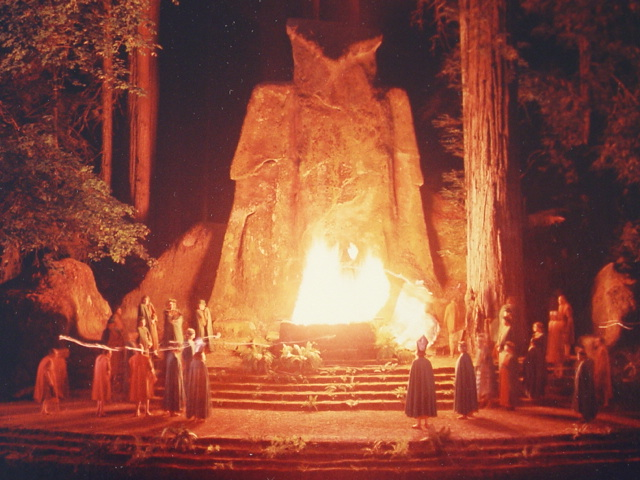
\includegraphics[width=\textwidth]{images/cremation_of_care.jpg}
		\end{frame}
	
		\begin{frame}
			\frametitle{Challenge One - Corpus Results}
			\centering
			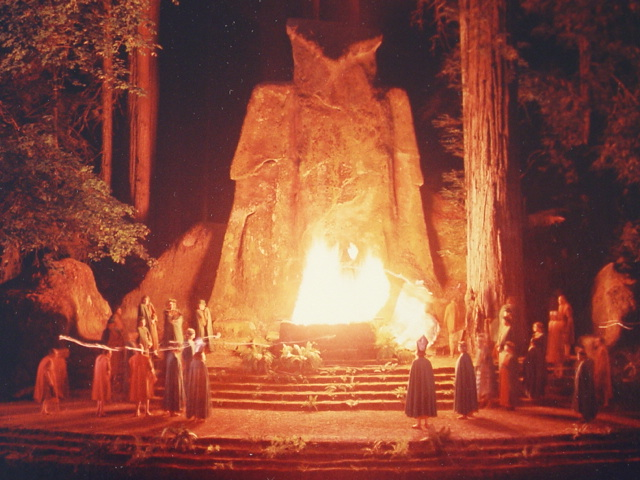
\includegraphics[scale=0.2]{images/cremation_of_care.jpg}
			\begin{itemize}
				\item Is this a religious ceremony?
				\item That looks very interesting, don't you think?
				\item What are they all gathered for?
				\item What are these people gathered for?
				\item Is this a satanic ritual?
			\end{itemize}
		\end{frame}
	
		\begin{frame}
			\frametitle{Challenge Two - Setup}
			Please go to: and enter in the code:
		\end{frame}
	
		%protests |	What are the people demonstrating about?---What rally are they attending?---What are these people protesting?---What are they protesting?---Who is in the gray jacket? |	A large crowd of egyptian protestors---A crowd is collected together as a mob---A crowd of protesters with one man standing tall---A large crowd of people protesting---A large group of men who seem to be protesting
		
		
		\begin{frame}
			\frametitle{Challenge Two}
			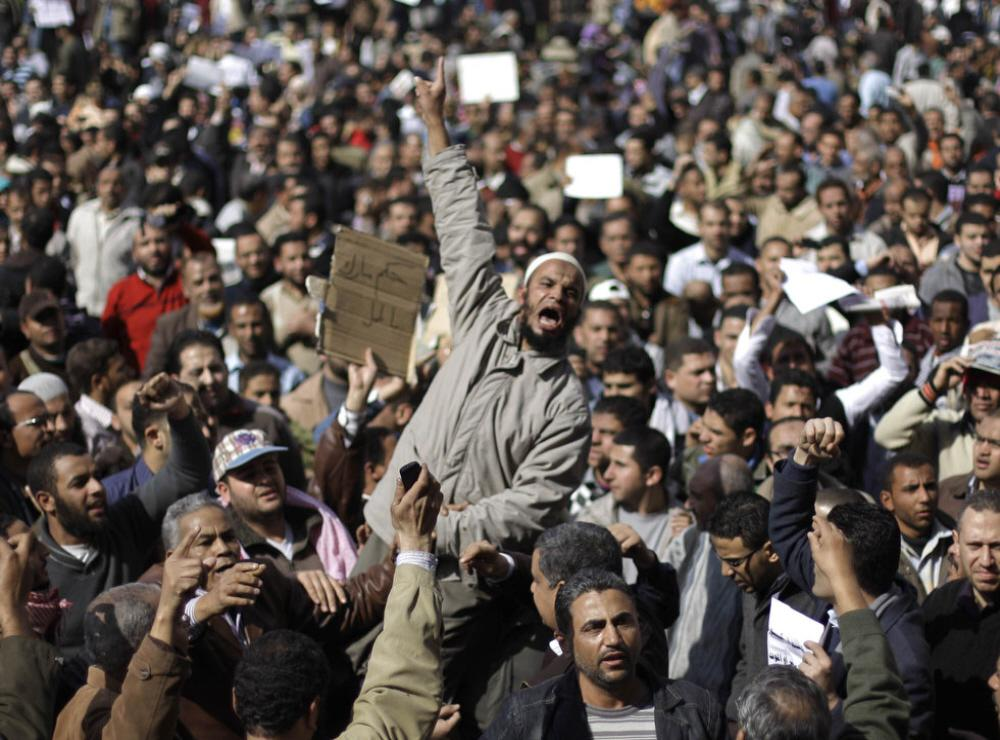
\includegraphics[width=\textwidth]{images/01c-egyptian-protests.jpg}
		\end{frame}
		
		\begin{frame}
			\frametitle{Challenge Two - Corpus Results}
			\centering
			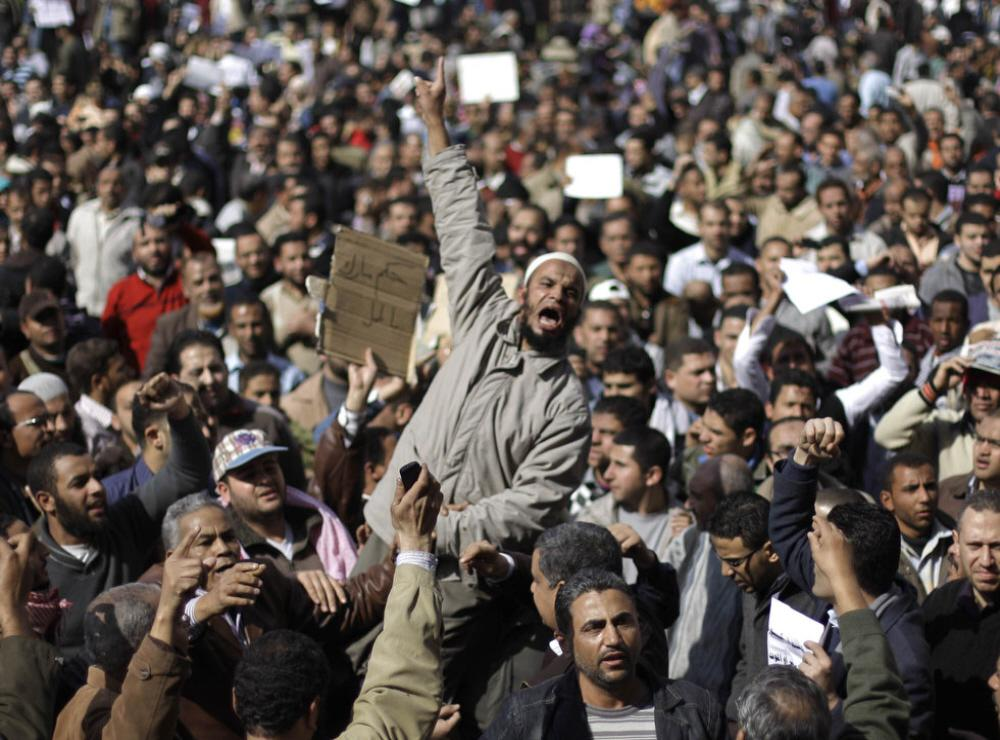
\includegraphics[scale=0.15]{images/01c-egyptian-protests.jpg}
			\begin{itemize}
				\item What are the people demonstrating about?
				\item What rally are they attending?
				\item What are these people protesting?
				\item What are they protesting?
				\item Who is in the gray jacket?
			\end{itemize}
		\end{frame}
	
		%TODO Introduce the task at hand - SARAH
		\subsection{The Authors' Objective}
		
			\begin{frame}
				\frametitle{}
				
			\end{frame}
	
	%TODO Image recognition. CNN intro and examples - RYAN
	\section{Image Recognition using a CNN}
		
		\begin{frame}
			\frametitle{What is Image Recognition?}
			
		\end{frame}
	
		\begin{frame}
			\frametitle{Image recognition and neural networks}
			\begin{figure}
				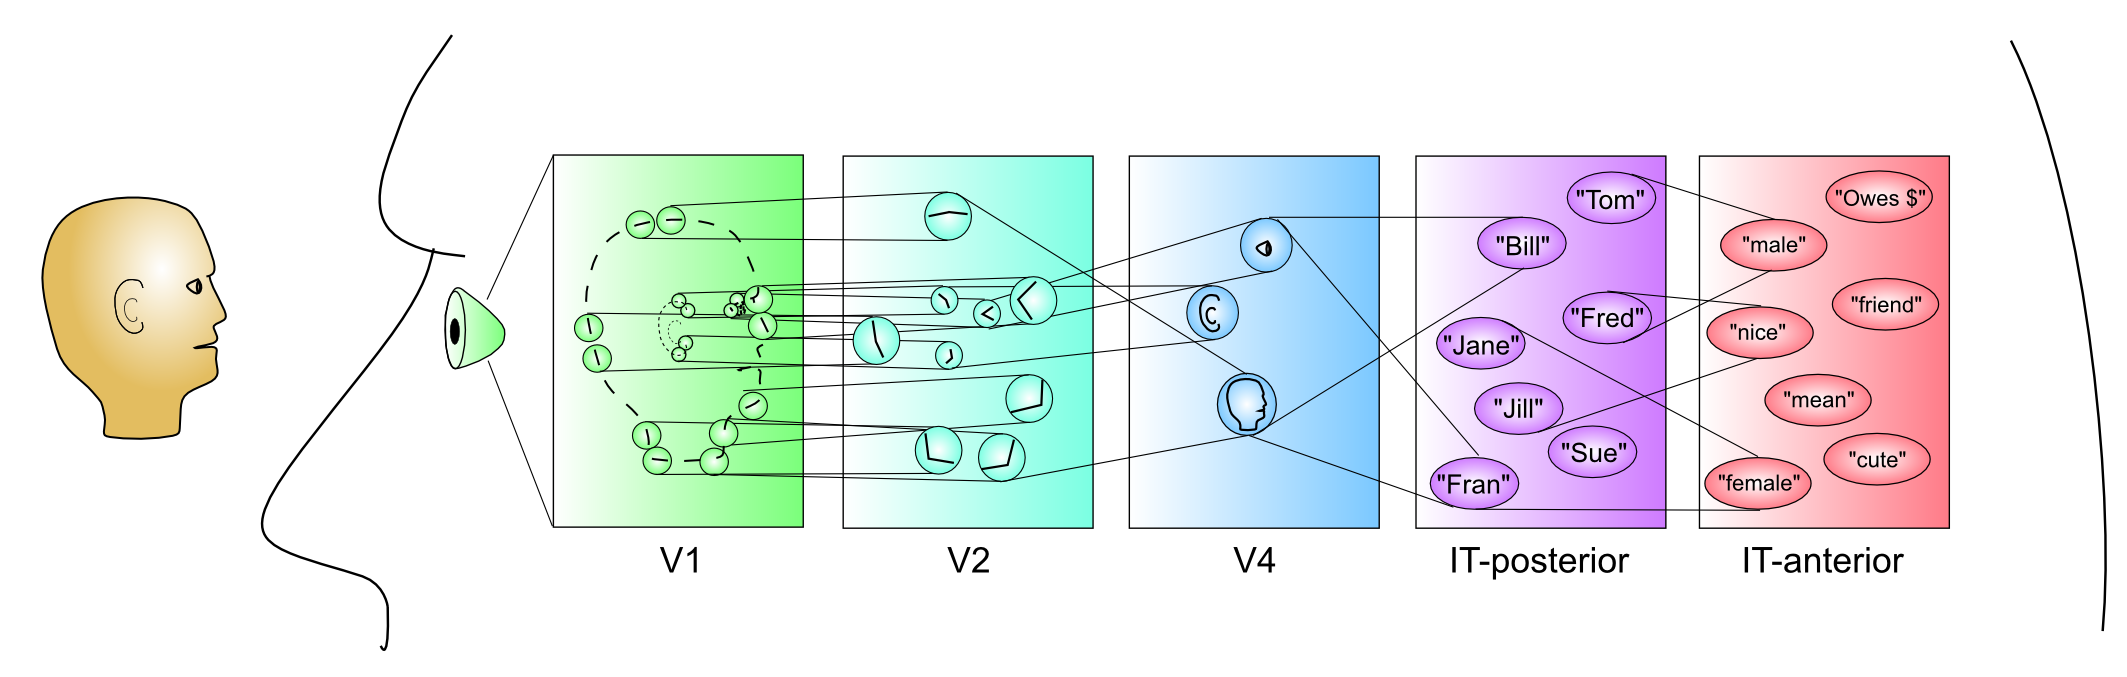
\includegraphics[width=\textwidth]{images/fig_category_hierarch_dist_reps.png}
				\caption{Visual network representation. \textit{Image from \href{https://grey.colorado.edu/CompCogNeuro/index.php/CCNBook/Networks}{grey.colorado.edu}} \cite{ccn_path}}
			\end{figure}
		\end{frame}

		\begin{frame}
			\frametitle{Convolutional neural network}
			\begin{figure}
				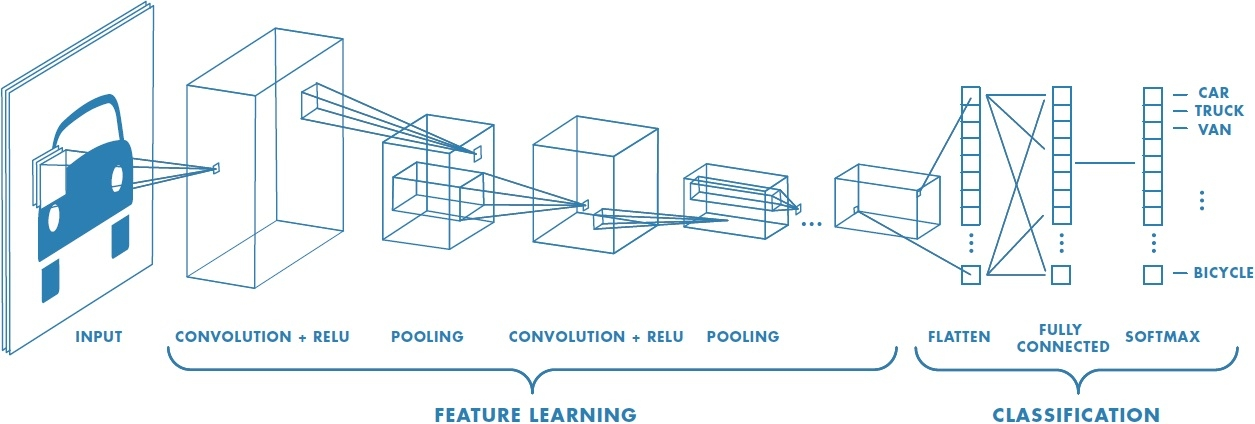
\includegraphics[width=\textwidth]{images/cnn2.jpg}
				\centering
				\caption{CNN representation. \textit{Image from \href{https://blog.floydhub.com/building-your-first-convnet/}{blog.floydhub.com/building-your-first-convnet}} \cite{first_cnn}}
			\end{figure}
		\end{frame}
		
		\begin{frame}
			\frametitle{CNN visualized}
			\begin{figure}
				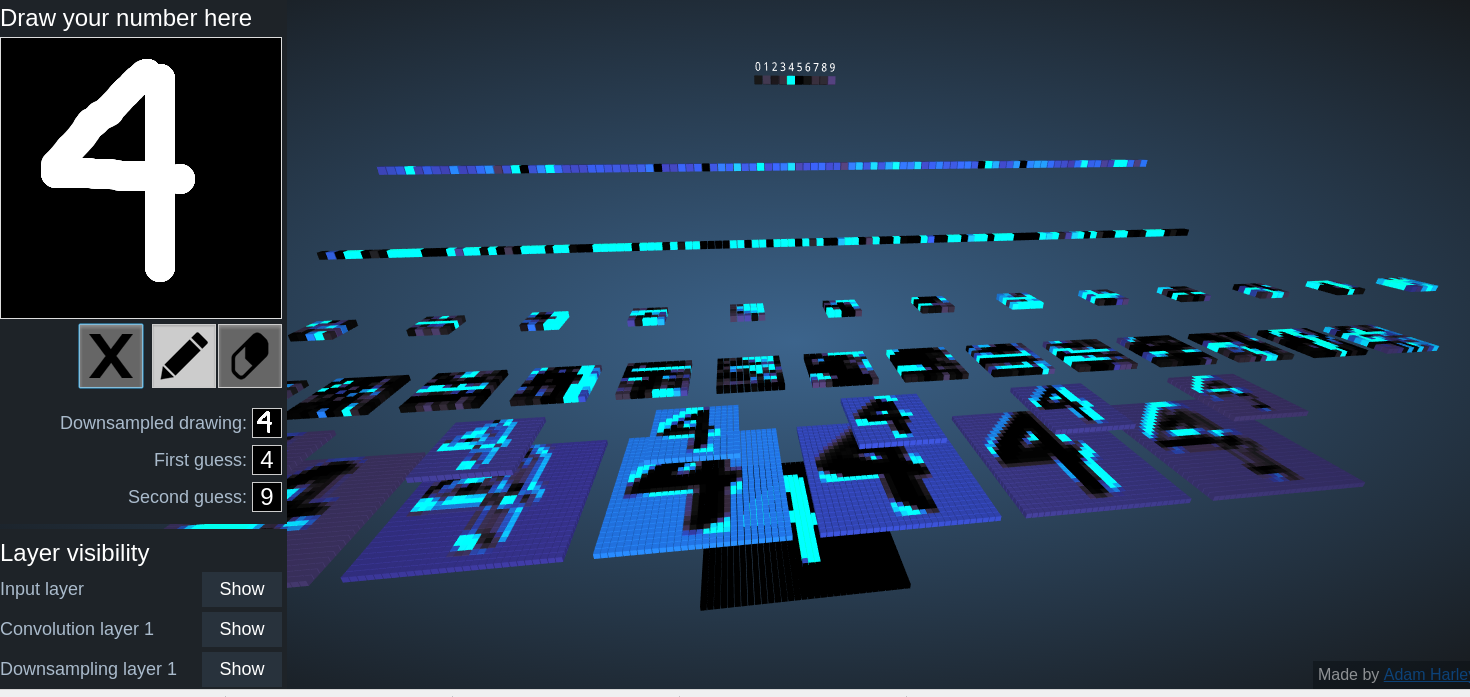
\includegraphics[width=\textwidth]{images/cnn_visual.png}
				\centering
				\caption{CNN visualized. \textit{Image from \href{http://scs.ryerson.ca/~aharley/vis/conv/}{scs.ryerson.ca/}} \cite{harley2015isvc}}
			\end{figure}
			
		\end{frame}
	
		\begin{frame}
			\frametitle{Why Does It Work Well for Images?}
			
		\end{frame}
	
	%TODO Talk about datasets and give examples and information about them. Mturk etc - SARAH
	\section{Datasets}
		
		\begin{frame}
			\frametitle{}
			
		\end{frame}
	
		\subsection{MS COCO}
			
			\begin{frame}
				\frametitle{}
				
			\end{frame}
		
		\subsection{Bing}
			
			\begin{frame}
				\frametitle{}
				
			\end{frame}
		
		\subsection{Flicker}
			
			\begin{frame}
				\frametitle{}
				
			\end{frame}
	
	\section{Generative Models}
		
		\begin{frame}
			\frametitle{Generative Models}
			\begin{center}
				
\includegraphics[scale=.3]{images/captionbot.jpg}
			\end{center}
			\begin{block}{Caption Bot \cite{fang2015captions}}
				\href{https://www.captionbot.ai/}{captionbot.ai} was used throughout this paper to automatically generate captions. It is a Microsoft project based on the \href{https://azure.microsoft.com/en-us/services/cognitive-services/computer-vision/}{Computer Vision API}, \href{https://azure.microsoft.com/en-us/services/cognitive-services/emotion/}{Emotion API}, and \href{https://azure.microsoft.com/en-us/services/cognitive-services/bing-image-search-api/}{Bing Image Search API}.
			\end{block}
		\end{frame}
	
		\begin{frame}
			\frametitle{Caption Bot example}
			\begin{center}
				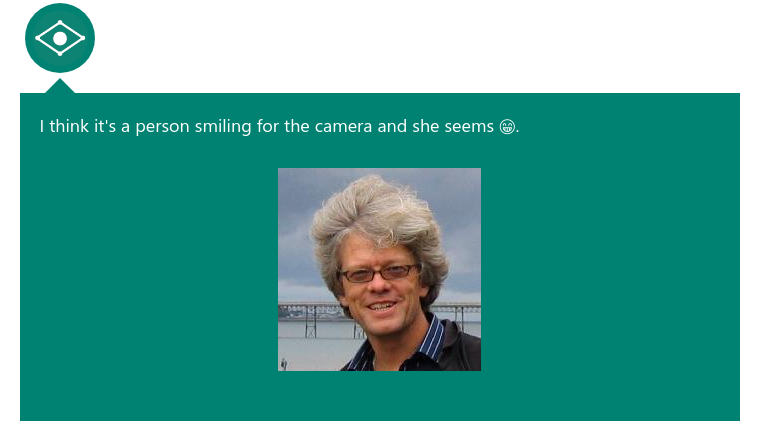
\includegraphics[width=\textwidth]{images/caption_detmar.png}
			\end{center}
		\end{frame}
	
		\begin{frame}
			\frametitle{Computer Vision API example}
			\begin{center}
				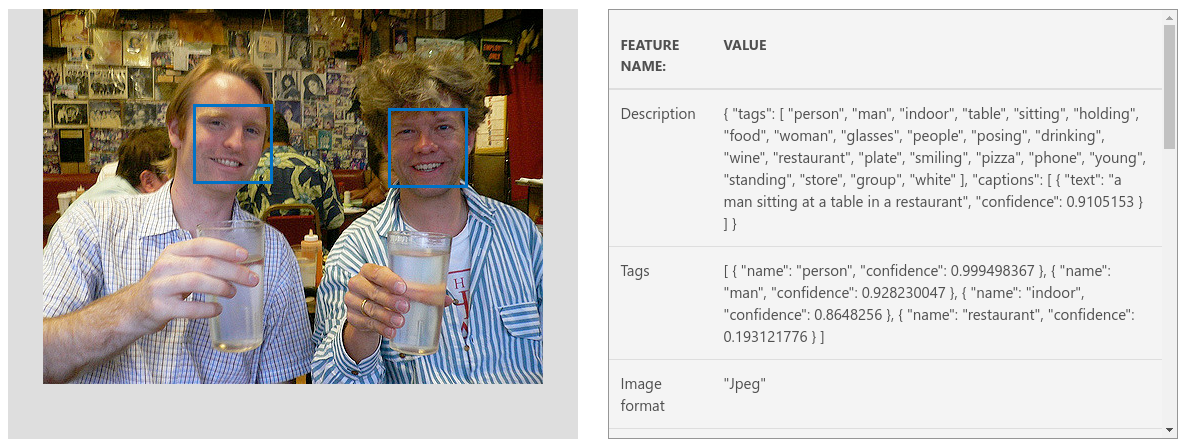
\includegraphics[width=\textwidth]{images/detmar_api.png}
			\end{center}
			\begin{itemize}
				\footnotesize{
					\item Description	{ "tags": [ "person", "man", "indoor", "table", "sitting", "holding", "food", "woman", "glasses", "people", "posing", "drinking", "wine", "restaurant", "plate", "smiling", "pizza", "phone", "young", "standing", "store", "group", "white" ], "captions": [ { "text": "a man sitting at a table in a restaurant", "confidence": 0.9105153 } ] }
					\item Faces	[ { "age": 25, "gender": "Male", "faceRectangle": { "top": 94, "left": 149, "width": 79, "height": 79 } }, { "age": 33, "gender": "Male", "faceRectangle": { "top": 97, "left": 343, "width": 79, "height": 79 } } ]
				}
			\end{itemize}
		\end{frame}
	
		%TODO Generative models melm, lstm, grnn - RYAN
		\subsection{Maximum Entropy Language Model}
			
			\begin{frame}
				\frametitle{MELM}
				
			\end{frame}
		
		\subsection{Long Short-Term Memory}
			
			\begin{frame}
				\frametitle{LSTM}
				
			\end{frame}
		
		\subsection{Gated Recurrent Neural Network}
			
			\begin{frame}
				\frametitle{GRNN}
				
			\end{frame}
	
	%TODO Retrieval models knn with closest semantic question - SARAH
	\section{Retrieval Model}
		
		\begin{frame}
			\frametitle{Retrieval Model}
			
		\end{frame}
		
		\subsection{K-Nearest Neighbor}
			
			\begin{frame}
				\frametitle{K-Nearest Neighbor}
				
			\end{frame}
			
			\begin{frame}
				\frametitle{BLEU}
				
			\end{frame}
	
	%TODO Evaluation. Pick out interesting stuff and examples of output - :(
	\section{Evaluation}
		
		\begin{frame}
			\frametitle{Evaluation}
			
		\end{frame}
	
		\begin{frame}
			\frametitle{BLEU \& METEOR}
			
		\end{frame}
	
	%TODO Discussion related things. Where it didnt work - BOTH
	\section{Discussion}
		
		\begin{frame}
			\frametitle{Discussion - Authors' Thoughts}
			
		\end{frame}
	
		%TODO Everyones least favorite part. Questions. Pick discussion questions for the groups - BOTH
		\subsection{Questions}
			
			\begin{frame}
				\frametitle{Questions}
				
			\end{frame}
	
	
	\section{References}
		
		\begin{frame}[allowframebreaks]
			\frametitle{References}
			\begin{footnotesize}
				\bibliographystyle{IEEE}
				\bibliography{BibMaster.bib}
			\end{footnotesize}
		\end{frame}

		
	\end{document}